%!TEX root = ../../lod-group1.tex
\subsection{Updating Movies}
\label{subsec_method_updating}

To ensure that the movies are always up to date, a scheduler is responsible to update the movies at certain repeading times.
The scheduler creates ``CrawlifyMatch'' tasks, which downloads the movie resource, which should be updated, triplifies it, matches it (if necessary) and stores the updated triples in the triple store.
Thereby, the scheduler distinguish between existing movies, which are released in the past from the current date, and coming soon movies, which will be released in the future.

\subsubsection{Adding coming soon movies}
The steps to add upcoming movies are:
\begin {enumerate}
	\item Get new movie resources.
	\item For each movie, download the new movie resource and triplify it.
	\item Delete all triples of the movie in the triple store in the corresponding graph, if the movie already exists.
	\item Load triples of an IMDb movie into the corresponding graph in the triple store. For the other resources, integrate the triples of the upcoming movie and store them in the corresponding graph.
\end{enumerate}

To get all new movies from IMDb, the scheduler crawls the ``Coming Soon'' page\footnote{\url{http://www.imdb.com/movies-coming-soon/2014-08/}} from the current month until the same month next year.
This page contains all new movies ids, which will be released in the time period crawled.
Having the new movie ids, the scheduler automatically can construct the new movie resource\footnote{\url{http://www.imdb.com/[id]}}, which can be crawled.

Freebase has an API, which the scheduler ask for all movies ids.
Afterwards, the scheduler filters the ids for those ids, which are unknown.
Thus, the scheduler gets all new movies.

TMDb offers a change set.
The scheduler requests the change API to get all movies, which recently changed.
Then, the scheduler can filter for movies, which are unkown and thus, which are new.

At OFDb the movies have increasing ids.
New movies published on the current day can be found under the following page \url{http://www.ofdb.de/view.php?page=neu&Kat=Film&Tage=1}.
So, the scheduler knows the highest newest movie id and also the last movie id of OFDb in the triple store.
All ids between these two are ids of new moives.
With the help of the ids, the scheduler can esaliy build the URL for the movie resource\footnote{\url{http://www.ofdb.de/film/[id]}} and crawl it.

To figure out how often the scheduler should add coming soon movies, IMDb's upcoming movie list was observed.
How many coming soon movies are daily added to IMDb is shown in Figure \ref{fig_coming_soon_movie}.
On a daily basis, the coming soon page from IMDb was crawled and the changes were recorded.
Almost every day, new movies are added or deleted from the IMDb coming soon list.
It is noticeable, that the most movies are published between Thursdays to Sundays on IMDb.

\begin{figure}[h!]
  \begin{center}
  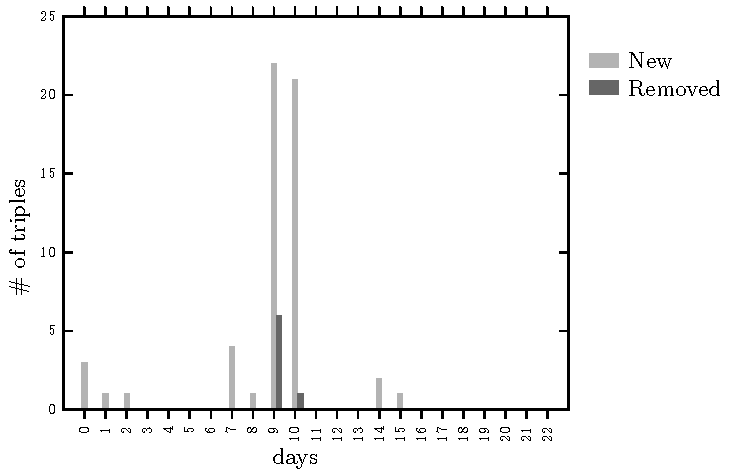
\includegraphics[width=0.8\textwidth]{images/updating_1.pdf}
  \end{center}
  \caption{Number of new coming soon movies, which are published on IMDb per day.}
  \label{fig_coming_soon_movie}
\end{figure}

From this observation we decided to update coming soon movies from IMDb daily.
TMDb and OFDb show a similar result, so that upcoming movies from these data sources are updated daily, too. The sandbox of Freebase, which is requested over the API, updates once a week. That is why, the upcoming movies from Freebase are updated only on weekly basis.

\subsubsection{Updating existing movies}
In Figure \ref{fig_new_movie} the number of changed triples of a new released movie from IMDb is displayed.
Therefor, a movie was crawled and triplified daily.
As you can seen, the movie frequently changes in the first days.
Also, the number of changing triples decreases with time.
Often changing triples are for example cast triple, links to images and videos, IMDb rating, charachter triples or taglines.

\begin{figure}[h!]
  \begin{center}
  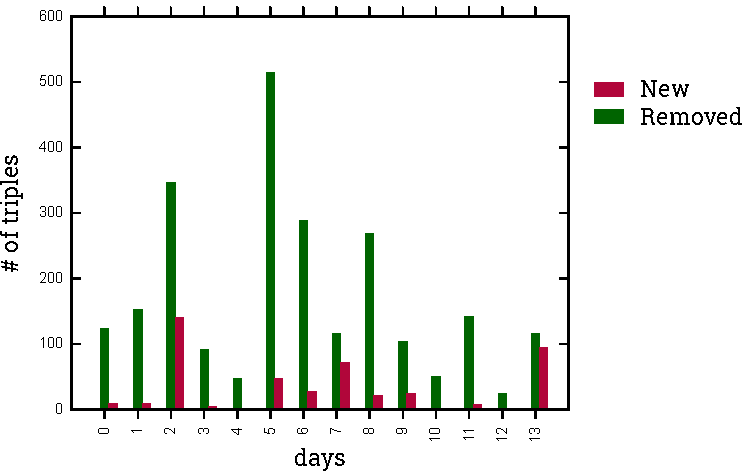
\includegraphics[width=0.8\textwidth]{images/updating_2.pdf}
  \end{center}
  \caption{Number of triples, which change in the first days of a new released movie from IMDb.}
  \label{fig_new_movie}
\end{figure}

Because a movie changes less the older the movie is, existings movies are divided into different categories.
Each category is updated at different frequencies (Table \ref{tab_updating_existing}).
\begin{table}[ht]
	\begin{center}
	\begin{tabular}{rl}
		\textbf{category of movie} & \textbf{frequency} \\ \hline
		one year old & weekly \\
		5 year old & monthly \\
		5 - 25 years old & yearly \\
		older than 25 years & never \\
	\end{tabular}
	\end{center}
	\caption{Frequency of updating existing movies}
	\label{tab_updating_existing}
\end{table}
If a category should be updated, the scheduler does the follwing steps:
\begin{enumerate}
	\item Find all movies, which should be updated regardless their originial data source.
	\item For each of these movies, get the updated movie resource and triplify it.
	\item Delete all triples of the movie in the triple store in the corresponding graph.
	\item Load the new triples into the corresponding graph in the triple store.
\end{enumerate}
Because the movies are stored in different graphs depending on their originial data source, the scheduler knows, where to find the movie resource in the web.
The originial resource of a movie is stored in a \emph{sameAs} triple.
Deleting the existing triples and storing the new downloaded triples, ensures that no conflicting information is stored of a resource.